\documentclass[letterpaper, 12pt, oneside]{book}
\usepackage[top=1in, bottom=1in,margin=1in]{geometry}
\usepackage{lscape}
\usepackage{setspace}
\usepackage{longtable}
\usepackage{amsmath,amsthm,amsfonts, amssymb}
% \usepackage{mathptmx} % times new roman 
\usepackage{newtxtext,newtxmath} % times new roman font throughout the paper
% \usepackage{newtxtext,newtxmath}
% For python environments
% \usepackage{listings}
% \usepackage{fontspec}
% \usepackage{minted}
\usepackage{cite}
\usepackage{wasysym}
\usepackage{textcomp}
\usepackage{comment}
\usepackage{titlesec}

\usepackage{lipsum}

\usepackage{tocloft}

%%%%%%%%%%% font settings %%%%%%%%%%%%%%%
% when setting 12 pt in \documentclass[letterpaper, 12pt, oneside]{book}
% \normalsize = 12pt
% \large = 14pt

%%%%%%%%%%%%%%%%%%%%%%%%%%%%%%%%%%%%%%%%%%%%%%

%%% change the spacing between the dots, in lists of Tables and Figures, Table of contents %%
\cftsetpnumwidth{1em} % make sure ..... goes all the way to page numbers
\renewcommand{\cftdotsep}{0}% Default is 4.5
% \renewcommand*{\cftfigdotsep}{0} % medium spacing for figures
% \renewcommand*{\cfttabdotsep}{0} % medium spacing for tables
%%%%%%%%%%%%%%%%%%%%%%%%%%%%%%%%%%%%%%%%%%%%%%%%%%%%%%%%%%%%%%%%%%

%%%%%%%%%%% formatting \tableofcontents %%%%%%%%
\renewcommand{\cftchapleader}{\cftdotfill{\cftdotsep}} % ...... for chapters
\renewcommand\cftchappagefont{\normalfont} % do not use bold page numbers
\renewcommand{\cftchapaftersnum}{.} % add . for chapters in tableofcontents
% \renewcommand{\cftchaptitlefont}{100pt} % this command seems be overwritten by titlesec
%%%%%%%%%%%%%%%%%%%%%%%%%%%%%%%%%%%%%%%%%%%%%%%%%%%%%%%%%%%%%%%%%%

%%%%%%%%%%% add Figure 1.x to \listoffigures %%%%%%%%%%%
\renewcommand{\cftfigpresnum}{\figurename~}
% \renewcommand{\cftfigaftersnum}{:} % add : after Figure, i.e., Figure: 
\addtolength{\cftfignumwidth}{3em}
\setlength{\cftfigindent}{0in} % indent spacing from left edge of paper to word `Figure` 
%%%%%%%%%%%%%%%%%%%%%%%%%%%%%%%%%%%%%%%%%%%%%%%%%%%%%%%%
%%%%%%%%%%% add Table 1.x to \listoftables %%%%%%%%%%%
\renewcommand{\cfttabpresnum}{\tablename~}
% \renewcommand{\cfttabaftersnum}{:} % add : after Table, i.e., Table: 
\addtolength{\cfttabnumwidth}{2.5em}
\setlength{\cfttabindent}{0in} % indent spacing from left edge of paper to word `Table` 
%%%%%%%%%%%%%%%%%%%%%%%%%%%%%%%%%%%%%%%%%%%%%%%%%%%%%%%%

\renewcommand{\contentsname}{\hspace{6.5cm}Table of Contents} % \hspace{6cm} is to make the title in the center
\renewcommand{\listtablename}{\hspace{7cm}List of Tables} % \hspace{6cm} is to make the title in the center
\renewcommand{\listfigurename}{\hspace{7cm}List of Figures} % \hspace{6cm} is to make the title in the center
\renewcommand{\cftloftitlefont}{\bfseries\large}
\renewcommand{\cfttoctitlefont}{\bfseries\large}
\renewcommand{\cftlottitlefont}{\bfseries\large}
% \renewcommand{\cftpartfont}{\normalfont\sffamily\bfseries}% \part font in ToC
\renewcommand{\cftchapfont}{\normalfont}    % \chapter font in ToC
\renewcommand{\cftsecfont}{\normalfont}           % \section font in ToC
\renewcommand{\cftsubsecfont}{\normalfont}        % \subsection font in ToC
\renewcommand{\cftsubsubsecfont}{\normalfont}       % \subsubsection font in ToC

% %%%%%%%%%%%% formatting Chapter/Section/Subsection titles
% the following lines are covered by the titlesec package
% \renewcommand\thesection{\thechapter.\arabic{section}} % remove '.', e.g., '1.1. Title' --> '1.1 Title'
% \renewcommand\thesubsection{\thesection.\arabic{subsection}} % remove '.', e.g., '1.1.1. Title' --> '1.1.1 Title'
% \renewcommand\thesubsubsection{\thesubsection.\arabic{subsubsection}} % remove '.', e.g., '1.1.1.1. Title' --> '1.1.1.1 Title'
% %%%%%%%%%%%%%%%%%%%%%%%%%%%%%%%%%%%%%%%%%%%%%%%%%%%%%%%%

% \usepackage{fontspec}
% \setmainfont{Times New Roman}

%\titleformat{\chapter}[display]
%  {\normalfont\bfseries\centering}{}{0pt}{\Large\thechapter. }

%\titleformat{\chapter}{\Large\bfseries\centering}{\thechapter. }{1em}{}
% \titleformat{\chapter}{\large\bfseries\centering}{\thechapter.}{1em}{}
\titleformat{\chapter}{\large\bfseries}{\thechapter.}{1em}{}
[\vspace{-3ex}
\rule{\textwidth}{1pt}]
% \titlespacing\chapter{0pt}{12pt plus 4pt minus 2pt}{0pt}
\titlespacing\chapter{0pt}{-0.5in}{0pt} % this command controls the margin

% \titlespacing{\chapter}{0pt}{-32pt}{1cm}% <-- CHANGE DONE HERE!!

\titleformat{\section}{\large\normalsize\bfseries}{\thesection}{1em}{}
\titlespacing\section{0pt}{12pt}{0pt}

\titleformat{\subsection}{\large\normalsize\bfseries}{\thesubsection}{1em}{}
\titlespacing\subsection{0pt}{12pt}{0pt}

\usepackage{subfig}

\usepackage{hyperref}
\hypersetup{
    colorlinks=true,
    linkcolor=black,
    filecolor=magenta,      
    urlcolor=cyan,
}
 
\urlstyle{same}

% \setsansfont{Calibri}
% \setmonofont{Consolas}

\usepackage[toc,page]{appendix}

% \usepackage{subcaption}
\usepackage{graphicx}
\graphicspath{{./fig/}}

\theoremstyle{plain}
\newtheorem{thm}{Theorem}
\newtheorem{lem}[thm]{Lemma}
\newtheorem{prop}[thm]{Proposition}
\newtheorem*{cor}{Corollary}

\theoremstyle{definition}
\newtheorem{defn}{Definition}
\newtheorem{conj}{Conjecture}
\newtheorem{exmp}{Example}

\theoremstyle{remark}
\newtheorem*{rem}{Remark}
\newtheorem*{note}{Note}

\newcommand{\se}[1]{{\textcolor{black}{{#1}}}}
\newcommand{\minimize}{\mathop{\textup{minimize}}}
\newcommand{\maximize}{\mathop{\textup{maximize}}}


\usepackage{algorithmic}
% \usepackage{graphicx}
\usepackage{textcomp}
\usepackage{caption}
\usepackage{wasysym}
\usepackage{float}
% \usepackage[sort,numbers]{natbib}
\usepackage{multirow}
\usepackage{nomencl}
\usepackage{textcomp}
\usepackage{array}
\usepackage{wrapfig}
\usepackage{tabularx}
\usepackage{etoolbox}
\renewcommand\nomgroup[1]{%
  \item[\bfseries
  \ifstrequal{#1}{A}{Abbreviations}{%
  \ifstrequal{#1}{B}{Terminology Definitions}{%
  \ifstrequal{#1}{C}{Symbols}{}}}%
]}

\setlength{\nomitemsep}{-\parsep}
\setlength\parindent{0pt}

\newcommand{\nomunit}[1]{%
\renewcommand{\nomentryend}{\hspace*{\fill}#1}}
\setlength{\parskip}{1em}
\pagestyle{plain}

% \makenomenclature
%\makeindex cas-dc-template-v4.nlo -s nomencl.ist -o cas-dc-template-v4.nls

%%%Author definitions
\def\tsc#1{\csdef{#1}{\textsc{\lowercase{#1}}\xspace}}
\tsc{WGM}
\tsc{QE}
\tsc{EP}
\tsc{PMS}
\tsc{BEC}
\tsc{DE}



\begin{document}
\pagenumbering{roman}
\begin{titlepage}
\centering
\quad
%\vspace{70pt}
\begin{LARGE}
\begin{spacing}{1}
\textbf{Full Title of the PSERC Project}
\end{spacing}
\end{LARGE}

\vspace{50pt}
\begin{large}
\textbf{Final Project Report}
\end{large}
\\
\vspace{40pt}
\begin{large}
\textbf{Project Team}\\
Jane Doe, Project Leader\\
XXXX University\\
\vspace{10pt}
John Doe\\
XXXX University
\end{large}
\\
\vspace{30pt}
\begin{large}
\textbf{Graduate Students}\\
% \vspace{10pt}
Full Name\\
XXXX State University\\
\vspace{10pt}
Full Name1\\
Full Name2\\
\vspace{5pt}
XXXX University
\end{large}
\\
%\vspace{50pt}
% \includegraphics[height=1.5in]{tamulogo.png}\hspace{50pt}
% \includegraphics[height=1.5in]{ercotlogo.png}
\vspace{60pt}
\begin{normalsize}
\textbf{PSERC Publication (number to be added by PSERC OFFICE)}\\
\vspace{20pt}
August 2020
\end{normalsize}
\end{titlepage}

% \textbf{For more Information about this Project, contact}\\
% \vspace{20pt}

% Dr. Le Xie \\ 
% % \label{par:dr_le_xie}
% Department of Electrical and Computer Engineering\\
% Texas A\&M University\\
% Phone: 979-845-7563\\
% Email: le.xie@tamu.edu
% % paragraph dr_le_xie (end)
\newpage
\noindent \textbf{For information about this project, contact:}
\vspace{10pt}

\noindent Jane Doe\\
XXXX University\\
School of Electrical, Computer and Energy Engineering\\
P.O. Box XXXXX\\
XXXX, New York, 14850\\
Phone: (123) 456-7890\\
Fax: (123) 456-7890  \\
Email: jane.due@xxxx.edu \\

\noindent \textbf{Power Systems Engineering Research Center}
\vspace{10pt}

\noindent The Power Systems Engineering Research Center (PSERC) is a multi-university Center conducting research on challenges facing the electric power industry and educating the next generation of power engineers. More information about PSERC can be found at the Center’s website: http://www.pserc.org. \\


\noindent \textbf{For additional information, contact:}
\vspace{10pt}

\noindent Power Systems Engineering Research Center\\
XXXXX University\\
XXXX Engineering Research Center\\
XXXXX, New York, 14850\\
Phone: (123) 456-7890\\
Fax: (123) 456-7890 \\


\noindent \textbf{Notice Concerning Copyright Material}
\vspace{10pt}

\noindent PSERC members are given permission to copy without fee all or part of this publication for internal use if appropriate attribution is given to this document as the source material. This report is available for downloading from the PSERC website.\\

\vspace{50pt}
\begin{center}
\textbf{\copyright  2020 XXXX University. All rights reserved.} 
\end{center}
% \thispagestyle{empty}
\pagenumbering{gobble} % this page is not counted in the report

\newpage
\pagenumbering{roman} % page count starts here
\begin{large}
\begin{center}
\textbf{Acknowledgments} 
\end{center}
\end{large}

%\chapter*{Acknowledgments}
We acknowledge the technical feedback from project advisors. 

\lipsum[3]

\newpage

\begin{large}
\begin{center}
\textbf{Executive Summary} 
\end{center}
\end{large}

%\chapter*{Executive Summary} 
% \begin{abstract}
%\begin{large}
\begin{spacing}{1.3}

\lipsum[5]


\newpage
\begin{large}
%\begin{center}
\textbf{Industry Advisors} 
%\end{center}
\end{large}$\quad$

\begin{table}[h]
  % \caption{caption here}
  % \label{tab:tablename}
  \centering

  \begin{tabular}{lll}
Full Name & ISO New England & xxxx.xxx@xxx.com \\
Full Name & CenterPoint & xxxx.xxx@xxx.com \\
\end{tabular}
\end{table}


\end{spacing}
%\end{large}

\begin{titlepage}
\centering
\quad \\
\quad \\
\quad \\
\quad \\
\quad \\
\quad \\
%\vspace{70pt}
% \begin{LARGE}
% \begin{spacing}{1}
\begingroup
    \fontsize{18pt}{20pt}\selectfont
    \textbf{Part I} \\
    \quad \\
    \quad \\
    \textbf{Full Title of the First Part of the Project}
\endgroup
% \end{spacing}
% \end{LARGE}


\vspace{80pt}

\begingroup
\fontsize{16pt}{20pt}\selectfont
John Doe\\
Full Name, Graduate Student\\
\quad \\
XXXX University    
\endgroup


\end{titlepage}

\newpage


% \begin{comment}
% \begin{large}
% \begin{center}
% \textbf{Table of Contents} 
% \end{center}
% \end{large}

% \makeatletter
% \renewcommand\tableofcontents{%
%     \@starttoc{toc}%
% }
% \makeatother
% \end{comment}

\newpage
\quad \vspace{-1in} % to make the title "Table of Contents" at top 1in margin
\tableofcontents

%\renewcommand{\cftafterloftitle{\newline}}
\newpage
\quad \vspace{-1in} % to make the title "List of Figures" at top 1in margin
\listoffigures

\newpage
\quad \vspace{-1in} % to make the title "List of Tables" at top 1in margin
\listoftables

% \begin{minted}[mathescape,
%                linenos,
%                numbersep=5pt,
%                gobble=2,
%                frame=lines,
%                framesep=2mm]{csharp}
%   string title = "This is a Unicode π in the sky"
%   /*
%   Defined as $\pi=\lim_{n\to\infty}\frac{P_n}{d}$ where $P$ is the perimeter
%   of an $n$-sided regular polygon circumscribing a
%   circle of diameter $d$.
%   */
%   const double pi = 3.1415926535
% \end{minted}

% \end{abstract}


\chapter[Short Chapter Title]{This is the full title of a Chapter}
\label{chap:chapter1}
This template is for a two-part PSERC Final report. If your report only has one part, then just use this one.
\section{Introduction} % (fold)
\label{sec:introduction}

\subsection{Background 1} % (fold)
\label{sub:background_1}

% subsection background_1 (end)

\subsection{Background 2} % (fold)
\label{sub:background_2}

% subsection background_2 (end)
% section introduction (end)


\chapter[Table, Figures, and Equations]{Basic \LaTeX~Elements}
\label{chap:chapter2}
Chapter \ref{chap:chapter2}, Section \ref{sec:text}, Subsection \ref{sub:background_1}.


\section{Equations} % (fold)
\label{sec:equations}
\subsection{Optimization Problem} % (fold)
\label{sub:optimization_problem}
\begin{subequations}
\begin{align}
\min~& \bm{f}(\bm{x}) \\
\text{s.t.}~& \bm{g}(\bm{x}) \le \bm{0}
\end{align}
\end{subequations}
% subsection optimization_problem (end)

\subsection{Multi-line Equations} % (fold)
\label{sub:multi_line_equations}
\begin{multline}
\alpha+\beta+2^{100} + \gamma = \alpha+\beta+2^{100} + \gamma = \alpha+\beta+2^{100} + \gamma = \\
\alpha+\beta+2^{100} + \gamma = \alpha+\beta+2^{100} + \gamma \\
= \alpha+\beta+2^{100} + \gamma 
\end{multline}
% subsection multi_line_equations (end)
% section equations (end)



\section{Figures} % (fold)
\label{sec:figures}
Figure \ref{fig:done}.

\begin{figure}[htbp]
  \centering
  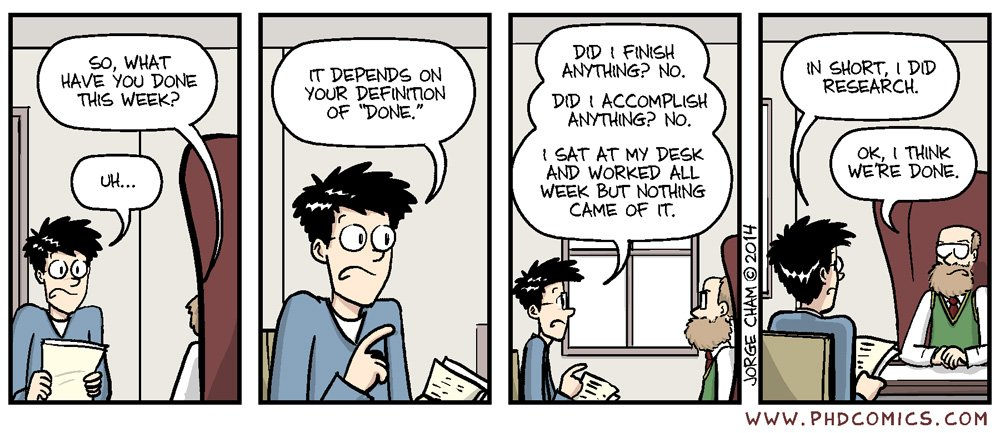
\includegraphics[width=\linewidth]{done.jpg}
  \caption{Done}
  \label{fig:done}
\end{figure}

\lipsum[1]
% section figures (end)

\section{Tables} % (fold)
\label{sec:tables}
Table \ref{tab:tablename}.

\begin{table}[tb]
  \caption{First Table}
  \label{tab:tablename}
  \centering

  \begin{tabular}{l|cc}
  \hline

  \hline
  \textbf{column 1} & \textbf{column 2} & \textbf{column 3} \\
  \hline
     & & \\
  \hline

  \hline
  \end{tabular}
\end{table}

\lipsum[1]
% section tables (end)

\section{Text} % (fold)
\label{sec:text}

\subsection{Citations} % (fold)
\label{sub:citations}
\begin{itemize}
\item Chapter \ref{chap:chapter2}, Section \ref{sec:text}, Subsection \ref{sub:background_1}.
\item Table \ref{tab:tablename}.
\item Figure \ref{fig:done}.
\end{itemize}
% subsection citations (end)

\subsection{itemize} % (fold)
\label{sub:itemize}

\begin{itemize}
\item \lipsum[1]
\item \lipsum[1]
\end{itemize}

\subsection{enumerate} % (fold)
\label{sub:enumerate}

\begin{enumerate}
\item \lipsum[1]
\item \lipsum[1]
\end{enumerate}
% section text (end)


\renewcommand\bibname{References}
\bibliographystyle{IEEEtran}
\bibliography{references}
% \bibliographystyle{plain}
% \bibliography{myreferences}

\end{document}



